\documentclass[aspectratio=169, 12pt]{beamer}
\usepackage[utf8]{inputenc}
\usepackage{utopia}
\usepackage{graphicx}
\usepackage{caption}
\usepackage{float}
\usepackage{subfig}
\usepackage[ruled,vlined]{algorithm2e}
\usepackage[export]{adjustbox}
\usefonttheme[onlymath]{serif}
\usepackage{amsmath, mathtools, bm}
\usepackage[backend=bibtex, style=verbose, sorting=ynt, dashed=false, maxnames=15]{biblatex}
\usepackage{tikz}
\bibliography{slides-bib}
\usepackage{multirow}
\usepackage{cellspace}
\usepackage{tcolorbox}

% Graphics scaling
\makeatletter
\def\ScaleIfNeeded{%
    \ifdim\Gin@nat@width>\linewidth
        \linewidth
    \else
        \Gin@nat@width
    \fi
}
\let\Oldincludegraphics\includegraphics
\gdef\includegraphics{
\@ifnextchar[{\Oldincludegraphics}{\Oldincludegraphics[width=\ScaleIfNeeded]}}
\makeatother

% Custom font sizes
\makeatletter
\newcommand\notsotiny{\@setfontsize\notsotiny{6.5}{7.1}}
\newcommand\supertiny{\@setfontsize\supertiny{3.6}{3.6}}
\newcommand\smallerthansmall{\@setfontsize\notsotiny{7.1}{7.5}}
\makeatother

% Colors
\definecolor{WHITE}{RGB}{255,255,255}
\definecolor{GrayText}{RGB}{67, 67, 67}
\definecolor{Yellow}{RGB}{254, 253, 249}
\definecolor{Black}{RGB}{0, 0, 0}
\definecolor{Blue}{RGB}{0, 0, 255}
\definecolor{Gray}{RGB}{150, 150, 150}
\definecolor{LightGray}{RGB}{192, 192, 192}
\definecolor{Orange}{RGB}{255, 146, 3}
\definecolor{SLIMorange}{RGB}{222, 160, 84}
\definecolor{DarkRed}{RGB}{150, 50, 57}
\definecolor{MyBlue}{RGB}{0, 142, 196}
\definecolor{MyGreen}{RGB}{16, 167, 120}
\definecolor{DarkGreen}{RGB}{39, 122, 43}
\definecolor{mydarkblue}{rgb}{0,0.08,0.45}

% Beamer template settings
\setbeamertemplate{caption}[numbered]
\setbeamertemplate{footline}[frame number]{}
\setbeamertemplate{navigation symbols}{}
\setbeamertemplate{title page}[default][left,colsep=-4bp,rounded=true,shadow=\beamer@themerounded@shadow]
\setbeamertemplate{itemize items}{\scriptsize $\blacktriangleright$}
\setbeamertemplate{itemize/enumerate body begin}{\small}
\setbeamertemplate{itemize/enumerate subbody begin}{}
\setbeamertemplate{bibliography item}{}
\setbeamertemplate{frametitle}{%
    \vspace{1em} % Adjust the vertical space before the frame title
    \insertframetitle
}

% Beamer colors and fonts
\setbeamercolor{title}{fg=GrayText}
\setbeamerfont{title}{size=\Large,parent=structure,series=\bfseries}
\setbeamercolor{frametitle}{fg=GrayText}
\setbeamerfont{frametitle}{family=\bfseries}
\setbeamerfont{frametitle}{size=\large}
\setbeamercolor{structure}{fg=Black}
\setbeamercolor{normal text}{fg=GrayText}
\setbeamerfont{institute}{size=\small}
\setbeamerfont{date}{size=\small}
\setbeamerfont{footnote}{size=\tiny}
\setbeamercolor{background canvas}{bg=}
\setbeamercolor{page number in head/foot}{fg=GrayText}

% Custom commands
\newcommand{\KL}{\mathbb{KL}}
\newcommand{\B}{\mathbf}
\newcommand{\Bs}{\boldsymbol}
\newcommand{\bn}{\boldsymbol{\epsilon}}
\DeclareMathOperator*{\argmax}{arg\,max}
\DeclareMathOperator*{\argmin}{arg\,min}
\newcommand*\mystrut[1]{\vrule width0pt height0pt depth#1\relax}

% Captions setup
\captionsetup[subfloat]{margin=1em}
\captionsetup[justification=centering, skip=2pt]{}
\captionsetup[subfigure]{labelformat=empty}
\setlength{\abovecaptionskip}{20pt plus 3pt minus 2pt}

% Avoid reference numbers
\makeatletter
\def\@makefnmark{}
\DeclareMathSizes{\f@size}{11.5}{7}{7}
\makeatletter

% Document settings
\setbeamersize{text margin left=7.5mm,text margin right=7.5mm}

%------------------------------------------------------------
\begin{document}

\title[]
{Hierarchical clustering}

\subtitle{\large A general lattice theory perspective}

\author[shortname]{\normalsize \\
    Ali Siahkoohi\inst{1}, Joonas Ilmavirta\inst{2}, and Maarten V. de Hoop\inst{1}}
\institute[shortinst]{\footnotesize
    \inst{1}Department of Computational Applied Mathematics and Operations Research, Rice University \\[0.2em]
    \inst{2} Department of Mathematics and Statistics, University of Jyväskylä}
\date{\footnotesize\today}


\frame[plain]{\titlepage}


% ---------------------------------------------------------
\begin{frame}

    \bigskip
    \bigskip

    \centerline{\large\textbf{``Flat'' clustering}}

    \bigskip
    \bigskip

    \centerline{partitioning of data points into a fixed number of sets}

\end{frame}


% ---------------------------------------------------------
\begin{frame}

    \bigskip
    \bigskip

    \centerline{\large\textbf{The impossibility theorem of flat clustering}}

    \bigskip
    \bigskip

    \centerline{no clustering function simultaneously satisfies}

    \medskip

    \centerline{scale invariance, richness, and consistency\footfullcite{Kleinberg_2002}}

\end{frame}



% ---------------------------------------------------------
\begin{frame}

    \bigskip
    \bigskip

    \centerline{\large\textbf{Hierarchical clustering}}

    \bigskip
    \bigskip

    \centerline{family of partitionings of data points with varying degrees of ``granularity''}

    \footfullcite{JMLR:v18:15-376,}

    \begin{figure}
        \centering
        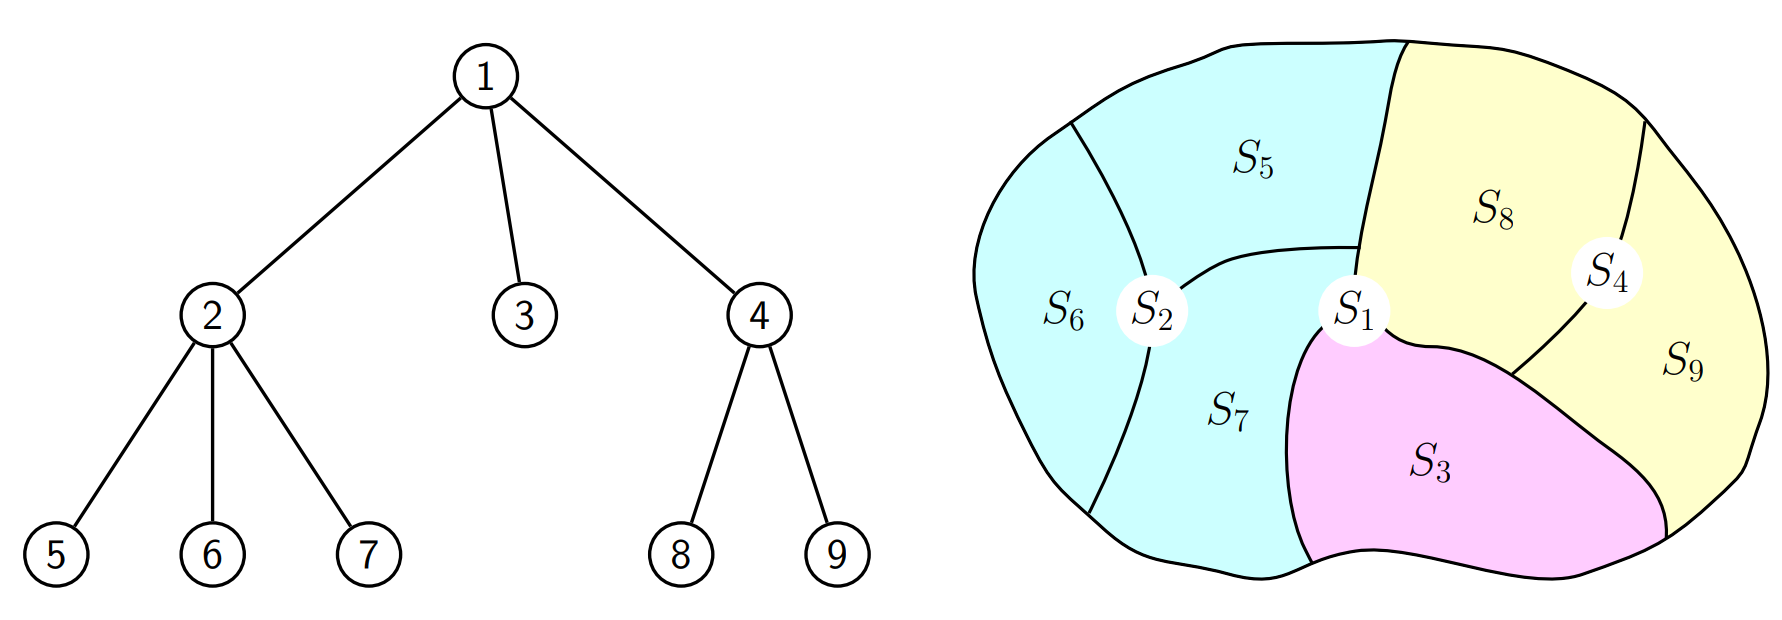
\includegraphics[width=0.6\textwidth, center]{figures/flat_vs_hc.png}
    \end{figure}

\end{frame}


% ---------------------------------------------------------
\begin{frame}


    \vspace*{-.55cm}

    \centerline{\large\textbf{Hierarchical clustering}}

    \bigskip
    \bigskip

    \centerline{relaxation of flat clustering: not restricted to a fixed number of clusters}

    \bigskip

    \centerline{no obstruction to existence (unlike flat clustering) \footfullcite{CarlssonEtAl_2010} \footfullcite{MoseleyEtAl_2017} \footfullcite{LaenenEtAl_2023}}

\end{frame}


% ---------------------------------------------------------
\begin{frame}

    \frametitle{Current hierarchical clustering algorithms}

    \begin{itemize}
        \setlength{\itemindent}{-1em}
        \setlength\itemsep{0.5em}
        \item[] {\color{DarkGreen} yield expected outcomes when applied to data with clear hierarchical structure}
        \item[] {\color{DarkRed} little is known theoretically when dealing with data with ambiguous discrete structure}
        \item[]  {\color{DarkRed} impose unnecessary constraints on solution, e.g.}
            \begin{itemize}
                \setlength{\itemindent}{-1.5em}
                \setlength\itemsep{0.5em}
                \item[\scriptsize\color{DarkRed}$\blacktriangleright$] {\color{DarkRed} tree (hyperbolic) metric embedding}
                \item[\scriptsize\color{DarkRed}$\blacktriangleright$] {\color{DarkRed} binary tree structure, e.g., single/average/complete linkage}
                \item[\scriptsize\color{DarkRed}$\blacktriangleright$] {\color{DarkRed} ultrametricity}
            \end{itemize}
    \end{itemize}


    \footfullcite{10.1145/3534678.3539378} \footfullcite{NEURIPS2019_b865367f} \footfullcite{NEURIPS2020_093f65e0}


\end{frame}

% ---------------------------------------------------------
\begin{frame}

    \bigskip
    \bigskip

    \centerline{\large\textbf{A lattice-theoretic framework for hierarchical clustering}}

    \bigskip
    \bigskip

    \centerline{drawing inspiration from the work in cognitive psychology}

    \medskip

    \centerline{stripping away unnecessary constraints and exploring the full solution space}

    \footfullcite{ReitmanRueter_1980} \footfullcite{Hirtle_1982}

\end{frame}


% ---------------------------------------------------------
\begin{frame}

    \frametitle{Outline}

    \begin{itemize}
        \setlength{\itemindent}{-1em}
        \setlength\itemsep{0.5em}
        \item[] hierarchical clustering in the context of lattice theory
            \begin{itemize}
                \setlength{\itemindent}{-1.5em}
                \setlength\itemsep{0.3em}
                \item lattice theory
                \item the lattice of partition space
                \item hierarchical clustering as chain inference
            \end{itemize}
        \item[] information-theoretical energy landscape over the lattice of partitions
            \begin{itemize}
                \setlength{\itemindent}{-1.5em}
                \setlength\itemsep{0.3em}
                \item minimum description length generative models
                \item optimal chain inference
            \end{itemize}
        \item[] computational heuristics
        \item[] remaining challenges
    \end{itemize}


\end{frame}

% ---------------------------------------------------------
\begin{frame}

    \vspace*{0.2cm}

    \begin{definition}{}

        \bigskip

        a \textbf{lattice} $L$ is a set $X$ together with a relation $\leq$ that satisfies the following properties:
        \begin{enumerate}
            \item $\leq$ is a partial ordering, i.e., for all $x, y, z \in X$:
                  \begin{itemize}
                      \item $x \leq x$
                      \item $x \leq y$ and $y \leq x \Rightarrow x = y$
                      \item $x \leq y$ and $y \leq z \Rightarrow x \leq z$
                  \end{itemize}
            \item every pair of elements $x, y \in X$ has a unique least upper bound, i.e., join, denoted by $x \cup y$
            \item every pair of elements $x, y \in X$ has a unique greatest lower bound, i.e., meet, denoted by $x \cap y$
        \end{enumerate}

    \end{definition}

    \footfullcite{Birkhoff_1979}

\end{frame}

% ---------------------------------------------------------
\begin{frame}

    \begin{definition}

        \bigskip


        a \textbf{partition} of set $X$ is a collection $\mathcal{P}$ of non-empty subsets of $X$ such that:

        \medskip

        \begin{itemize}
            \item every element of $X$ belongs to exactly one subset in $\mathcal{P}$.
            \item the union of all subsets in $\mathcal{P}$ equals $X$, i.e., $\bigcup_{A \in \mathcal{P}} A = X$.
            \item any two distinct subsets in $\mathcal{P}$ are disjoint, i.e., $\forall \, A, B \in \mathcal{P}$, if $A \neq B$, then $A \cap B = \emptyset$.
        \end{itemize}
    \end{definition}

\end{frame}

% ---------------------------------------------------------
\begin{frame}

    \begin{tcolorbox}[colback=white,colframe=black,title=Definition]
        a \textbf{partition} of set $X$ is a collection $\mathcal{P}$ of non-empty subsets of $X$ such that:

        \medskip

        \begin{itemize}
            \item every element of $X$ belongs to exactly one subset in $\mathcal{P}$.
            \item the union of all subsets in $\mathcal{P}$ equals $X$, i.e., $\bigcup_{A \in \mathcal{P}} A = X$.
            \item any two distinct subsets in $\mathcal{P}$ are disjoint, i.e., $\forall \, A, B \in \mathcal{P}$, if $A \neq B$, then $A \cap B = \emptyset$.
        \end{itemize}
    \end{tcolorbox}

\end{frame}

% ---------------------------------------------------------
\begin{frame}

    \begin{definition}

        \bigskip

        the \textbf{lattice of partitions} of set $X$, denoted $\mathcal{L} (\Pi(X), \leq)$, is the set of all partitions of $X$ together with the relation $\leq$ such that for any two partitions $\mathcal{P}$ and $\mathcal{Q}$ of $X$, we say $\mathcal{P} \leq \mathcal{Q}$ if and only if for every $A \in \mathcal{P}$, there exists $B \in \mathcal{Q}$ such that $A \subseteq B$. This relation $\leq$ is called the \textbf{refinement ordering} on partitions.

        The set $\Pi(X)$ together with the refinement ordering $\leq$ forms a lattice that satisfies the following properties:

        \begin{enumerate}
            \item $\leq$ is a partial ordering on $\Pi(X)$.
            \item For any two partitions $\mathcal{P}$ and $\mathcal{Q}$ of $X$, their least upper bound (join) $\mathcal{P} \cup \mathcal{Q}$ is the coarsest partition that refines both $\mathcal{P}$ and $\mathcal{Q}$.
            \item For any two partitions $\mathcal{P}$ and $\mathcal{Q}$ of $X$, their greatest lower bound (meet) $\mathcal{P} \cap \mathcal{Q}$ is the finest partition that is refined by both $\mathcal{P}$ and $\mathcal{Q}$.
        \end{enumerate}
    \end{definition}

\end{frame}

\end{document}
